% Copyright 2004 by Till Tantau <tantau@users.sourceforge.net>.
%
% In principle, this file can be redistributed and/or modified under
% the terms of the GNU Public License, version 2.
%
% However, this file is supposed to be a template to be modified
% for your own needs. For this reason, if you use this file as a
% template and not specifically distribute it as part of a another
% package/program, I grant the extra permission to freely copy and
% modify this file as you see fit and even to delete this copyright
% notice. 

\documentclass{beamer}

% There are many different themes available for Beamer. A comprehensive
% list with examples is given here:
% http://deic.uab.es/~iblanes/beamer_gallery/index_by_theme.html
% You can uncomment the themes below if you would like to use a different
% one:
%\usetheme{AnnArbor}
%\usetheme{Antibes}
%\usetheme{Bergen}
%\usetheme{Berkeley}
%\usetheme{Berlin}
%\usetheme{Boadilla}
%\usetheme{boxes}
%\usetheme{CambridgeUS}
%\usetheme{Copenhagen}
%\usetheme{Darmstadt}
%\usetheme{default}
%\usetheme{Frankfurt}
%\usetheme{Goettingen}
%\usetheme{Hannover}
%\usetheme{Ilmenau}
%\usetheme{JuanLesPins}
%\usetheme{Luebeck}
%\usetheme{Madrid}
%\usetheme{Malmoe}
%\usetheme{Marburg}
%\usetheme{Montpellier}
%\usetheme{PaloAlto}
%\usetheme{Pittsburgh}
%\usetheme{Rochester}
%\usetheme{Singapore}
%\usetheme{Szeged}
%\usetheme{Warsaw}

\usepackage{amsmath}
\usepackage{textpos}
\usepackage{ulem}

\definecolor{BYUblue}{RGB}{0,31,69}
\definecolor{BYUgold}{RGB}{195,163,106}
\usecolortheme[RGB={0,31,69}]{structure} % BYU Blue

\definecolor{metric-PR}{RGB}{200,127,0}
\definecolor{metric-NE}{RGB}{51,51,255}
\definecolor{metric-OFI}{RGB}{204,0,0}
\definecolor{metric-IRO}{RGB}{0,102,51}

\usetheme{Frankfurt}
\setbeamercolor*{section in head/foot}{bg=BYUblue,fg=gray!25}
\setbeamercolor*{frametitle}{bg=BYUblue!50,fg=white!25}
\setbeamercovered{transparent}
\mode<all>

\DeclareMathOperator*{\argmax}{arg\,max}

\title{Demo}

%\subtitle{Optional Subtitle}

\author{Daqing Yi 
%\and Michael A. Goodrich \and Kevin D. Seppi
}


\institute
{
  Department of Computer Science\\
  Brigham Young University
}

\date[]{} 

\addtobeamertemplate{frametitle}{}{%
\begin{textblock*}{100mm}(0.9\textwidth,-1.2cm)

\includegraphics[width=1.1cm]{figure/BYU_logo.png}
\end{textblock*}}

\begin{document}

\begin{frame}
  \titlepage
\end{frame}

\begin{frame}{Outline}{Structure}
  \tableofcontents
  % You might wish to add the option [pausesections]
\end{frame}

\section{Environment}

\begin{frame}{World}{Gazebo simulator}

\begin{figure}
\centering
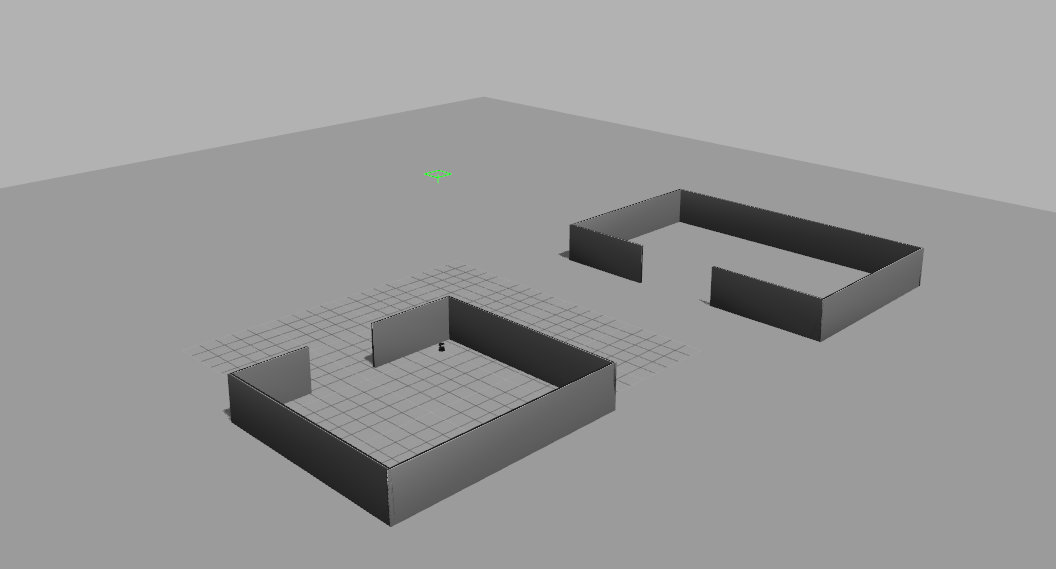
\includegraphics[width = 0.9\textwidth]{./screenshot/Gazebo.png}
%\caption{A coverage model.}
\end{figure}

\end{frame}

\begin{frame}{World}{World description}

\begin{columns}
\column{0.4\textwidth}
\begin{minipage}{\textwidth}
\begin{figure}
\centering
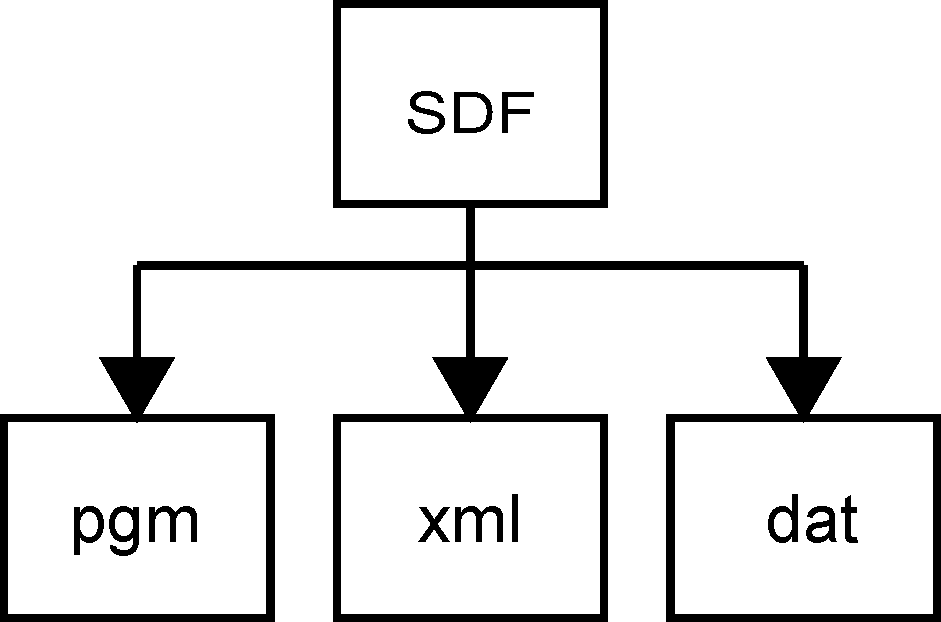
\includegraphics[width = \textwidth]{./figure/world_conversion.pdf}
\end{figure}
\end{minipage}

\column{0.6\textwidth}
\begin{minipage}{\textwidth}
\begin{itemize}
\item \textbf{SDF} - SDFormat(Gazebo) \\
\url{http://gazebosim.org/sdf.html}
\item \textbf{ppm} - bitmap description of the world 
\item \textbf{xml} - object description of the world
\item \textbf{dat} - binary description of the world
\end{itemize}
\end{minipage}
\end{columns}

\end{frame}

\section{Labeling}

\begin{frame}{Labeling}{Feature}

\begin{columns}
\column{0.6\textwidth}
\begin{figure}
\centering
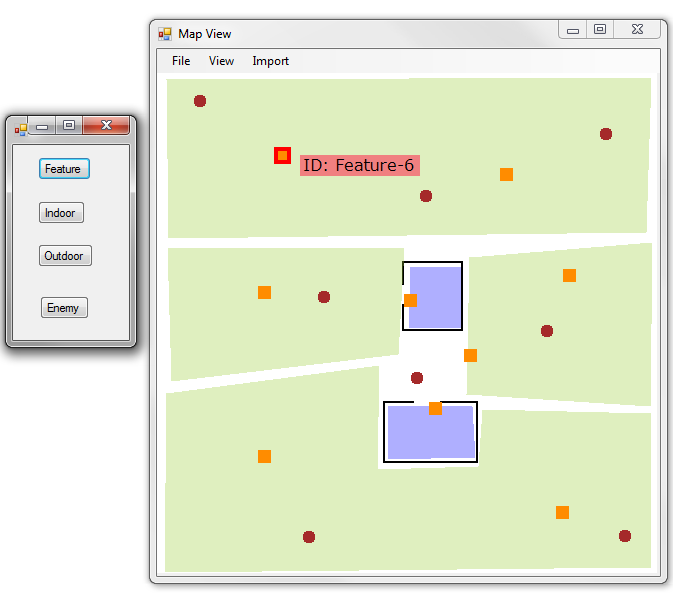
\includegraphics[width = \textwidth]{./screenshot/feature_label.png}
\end{figure}

\column{0.4\textwidth}
\begin{minipage}{\textwidth}
\begin{itemize}
\item Position
\item ID
\item Name
\end{itemize}
\end{minipage}
\end{columns}

\end{frame}

\begin{frame}{Labeling}{Indoor}

\begin{columns}
\column{0.6\textwidth}
\begin{figure}
\centering
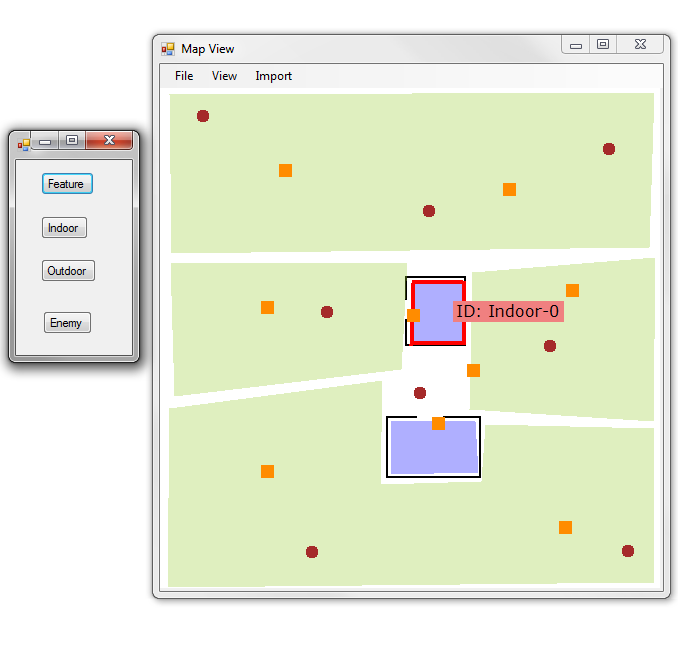
\includegraphics[width = \textwidth]{./screenshot/indoor_label.png}
\end{figure}

\column{0.4\textwidth}
\begin{minipage}{\textwidth}
\begin{itemize}
\item Vertex List
\item ID
\item Name
\end{itemize}
\end{minipage}
\end{columns}

\end{frame}

\begin{frame}{Labeling}{Outdoor}

\begin{columns}
\column{0.6\textwidth}
\begin{figure}
\centering
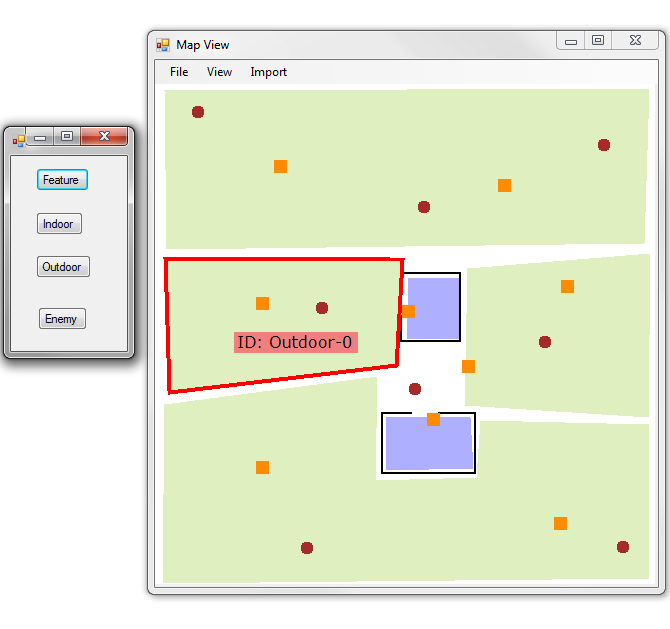
\includegraphics[width = \textwidth]{./screenshot/outdoor_label.png}
\end{figure}

\column{0.4\textwidth}
\begin{minipage}{\textwidth}
\begin{itemize}
\item Vertex List
\item ID
\item Name
\item Type
\end{itemize}
\end{minipage}
\end{columns}

\end{frame}

\begin{frame}{Labeling}{Enemy}

\begin{columns}
\column{0.6\textwidth}
\begin{figure}
\centering
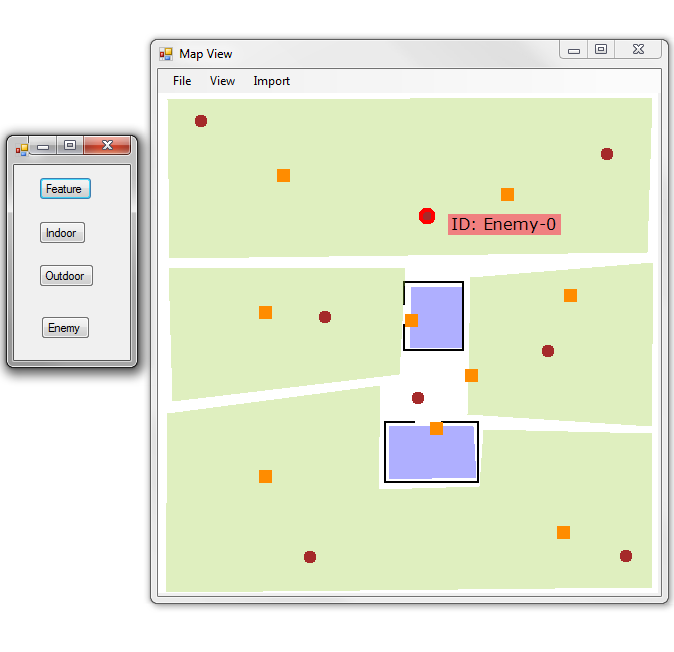
\includegraphics[width = \textwidth]{./screenshot/enemy_label.png}
\end{figure}

\column{0.4\textwidth}
\begin{minipage}{\textwidth}
\begin{itemize}
\item ID
\item Name
\item Position
\end{itemize}
\end{minipage}
\end{columns}

\end{frame}

\begin{frame}{Label data format}{XML}

\begin{columns}
\column{0.7\textwidth}
\begin{figure}
\centering
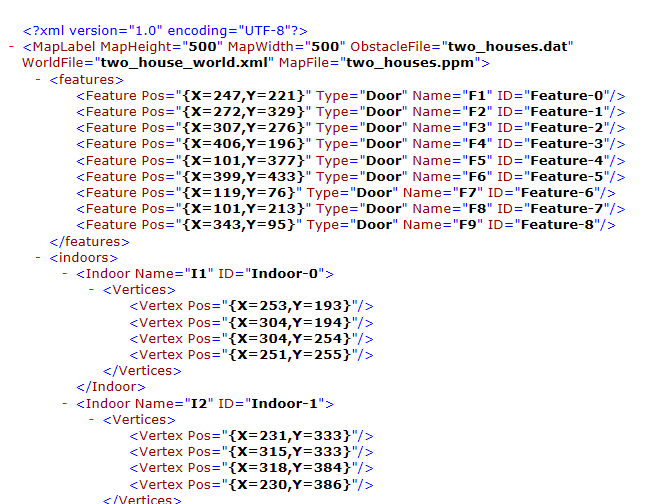
\includegraphics[width = \textwidth]{./screenshot/label_data_xml.png}
\end{figure}

\column{0.3\textwidth}
\begin{minipage}{\textwidth}
To be connected with RTCA robot perception.
\end{minipage}
\end{columns}

\end{frame}

\section{Planning}

\begin{frame}{Discretization}{Hexagonal map}

\begin{figure}
\centering
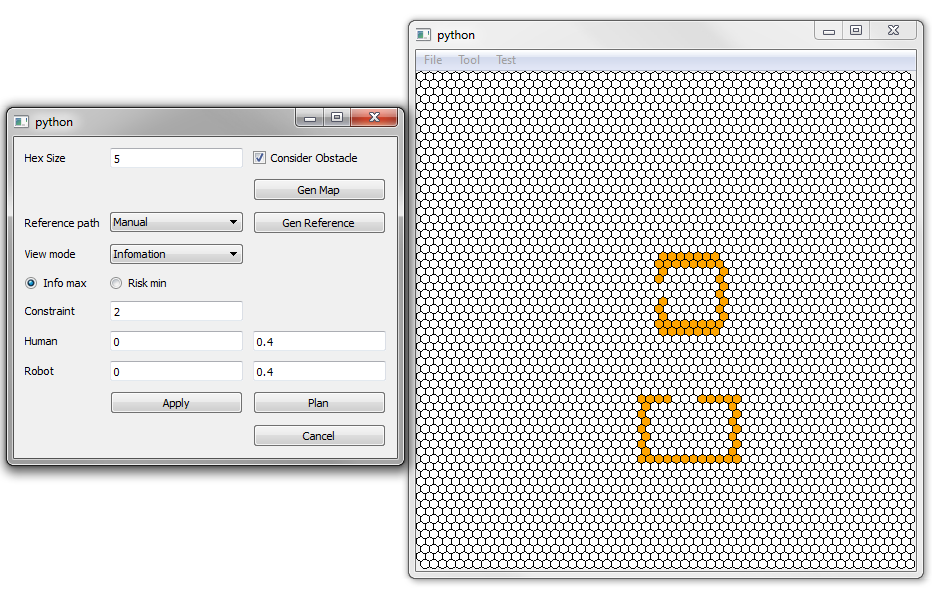
\includegraphics[width = 0.9\textwidth]{./screenshot/discretization.png}
\end{figure}

\end{frame}

\begin{frame}{View}{Information distribution}

\begin{columns}
\column{0.7\textwidth}
\begin{figure}
\centering
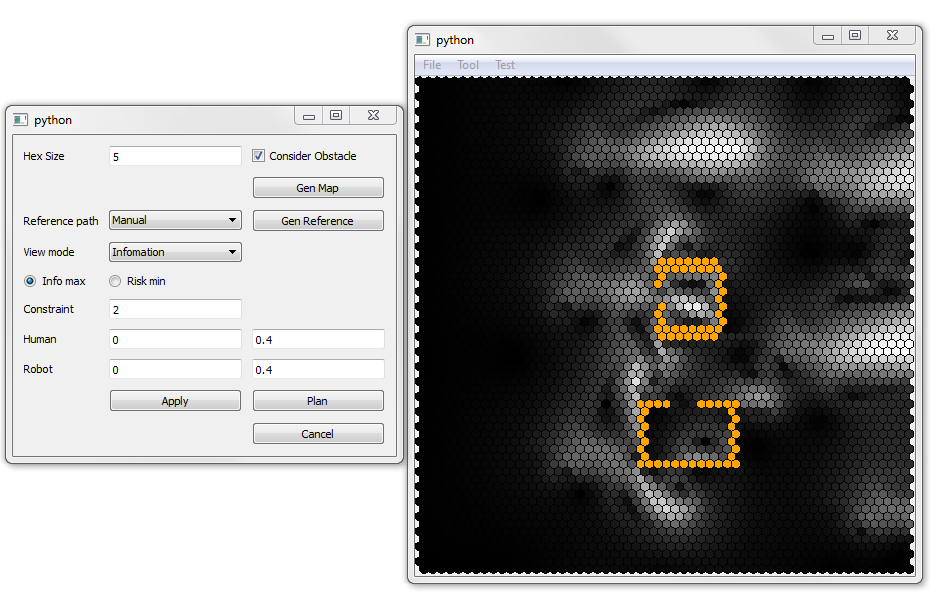
\includegraphics[width = \textwidth]{./screenshot/information_view.png}
\end{figure}

\column{0.3\textwidth}
\begin{minipage}{\textwidth}
\end{minipage}
\end{columns}

\end{frame}

\begin{frame}{View}{Enemy visibility}

\begin{columns}
\column{0.7\textwidth}
\begin{figure}
\centering
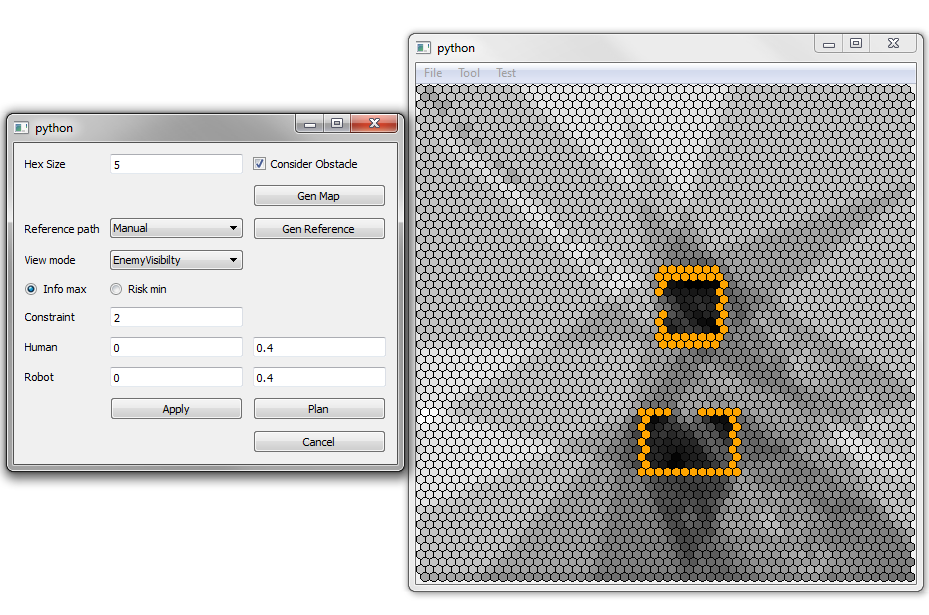
\includegraphics[width = \textwidth]{./screenshot/enemy_visibility_view.png}
\end{figure}

\column{0.3\textwidth}
\begin{minipage}{\textwidth}
\end{minipage}
\end{columns}

\end{frame}

\begin{frame}{View}{Position visibility}

\begin{columns}
\column{0.7\textwidth}
\begin{figure}
\centering
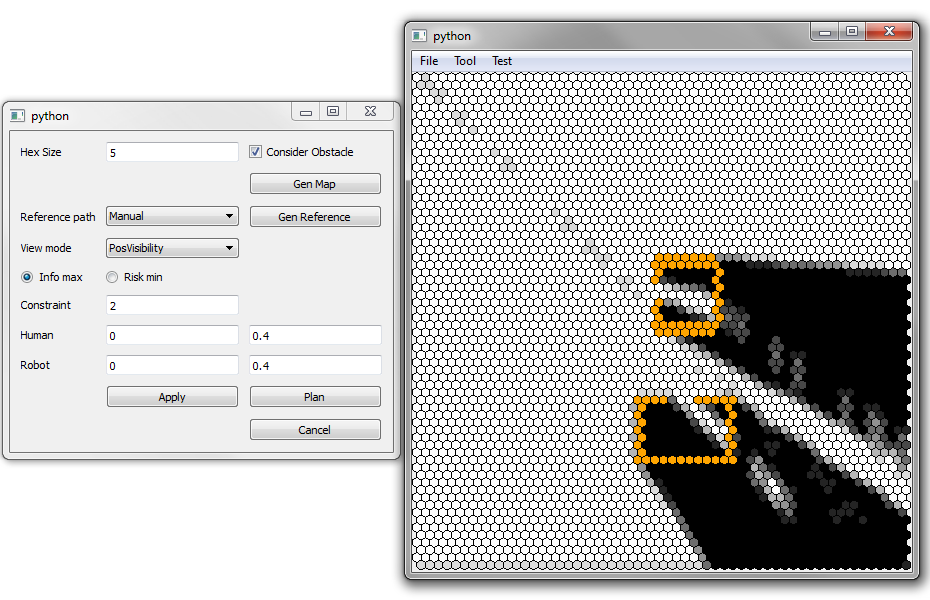
\includegraphics[width = \textwidth]{./screenshot/position_visibility_view1.png}
\end{figure}

\column{0.3\textwidth}
\begin{minipage}{\textwidth}
\end{minipage}
\end{columns}

\end{frame}

\begin{frame}{View}{Position visibility}

\begin{columns}
\column{0.7\textwidth}
\begin{figure}
\centering
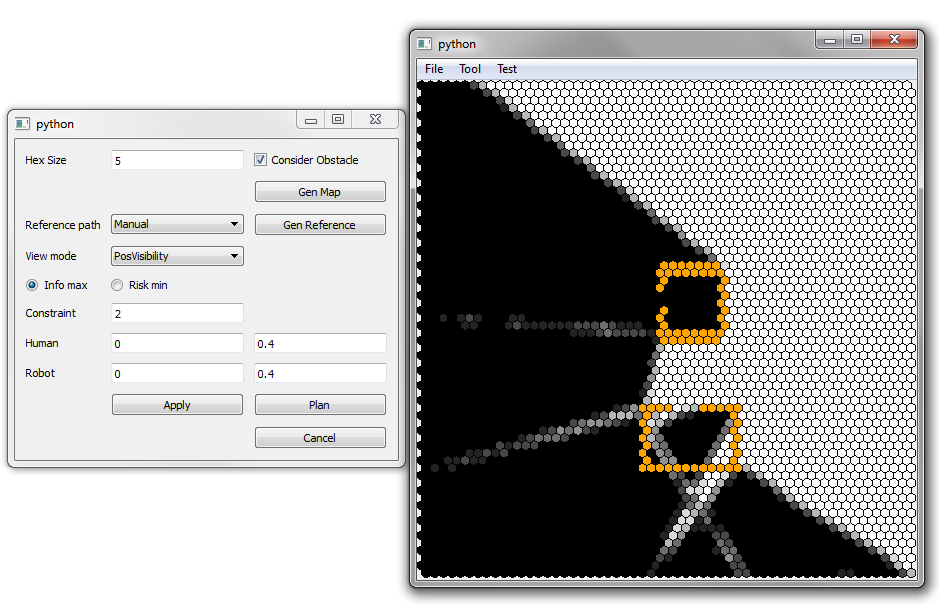
\includegraphics[width = \textwidth]{./screenshot/position_visibility_view2.png}
\end{figure}

\column{0.3\textwidth}
\begin{minipage}{\textwidth}
\end{minipage}
\end{columns}

\end{frame}

\begin{frame}{View}{Average visibility}

\begin{columns}
\column{0.7\textwidth}
\begin{figure}
\centering
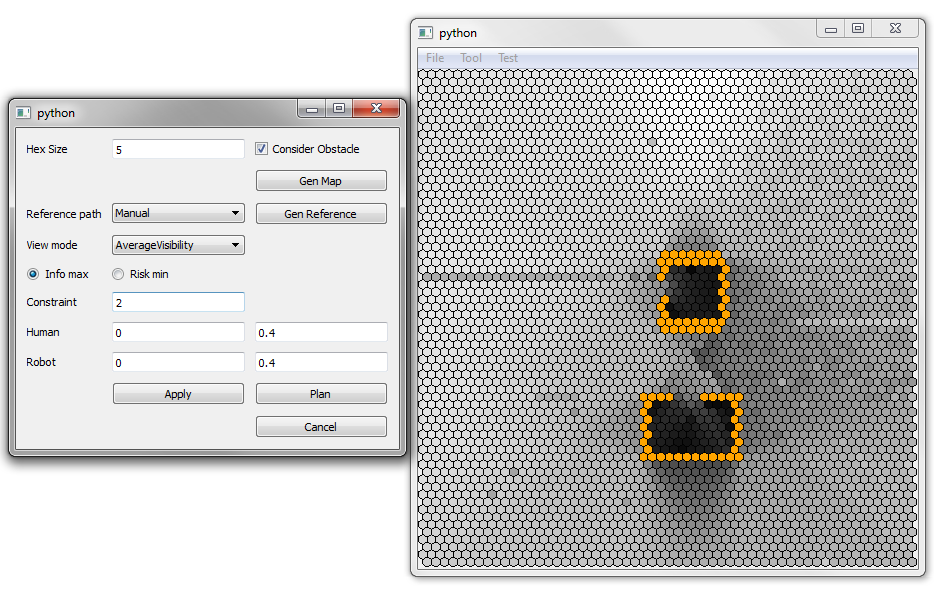
\includegraphics[width = \textwidth]{./screenshot/average_visibility_view.png}
\end{figure}

\column{0.3\textwidth}
\begin{minipage}{\textwidth}
\end{minipage}
\end{columns}

\end{frame}

\begin{frame}{Reference path}{Manual}

\begin{columns}
\column{0.65\textwidth}
\begin{figure}
\centering
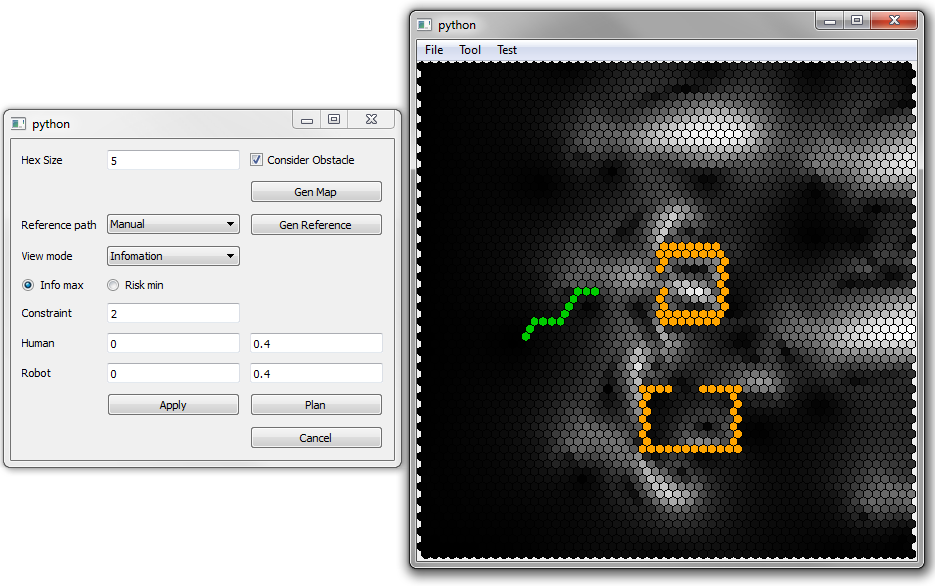
\includegraphics[width = \textwidth]{./screenshot/manual_reference_path.png}
\end{figure}

\column{0.35\textwidth}
\begin{minipage}{\textwidth}
\begin{figure}
\centering
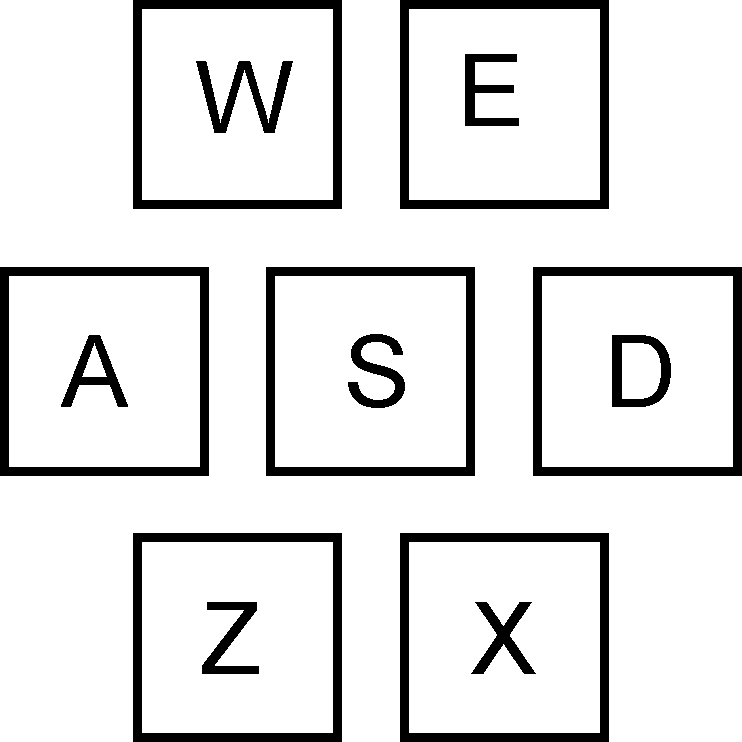
\includegraphics[width = .5\textwidth]{./figure/keyboard_op.pdf}
\end{figure}
\begin{itemize}
\item \textbf{W} - North West
\item \textbf{E} - North East
\item \textbf{A} - West 
\item \textbf{S} - Stay
\item \textbf{D} - East
\item \textbf{Z} - South West
\item \textbf{X} - South East
\end{itemize}
\end{minipage}
\end{columns}

\end{frame}

\begin{frame}{Reference path}{Quickly}

\begin{columns}
\column{0.65\textwidth}
\begin{figure}
\centering
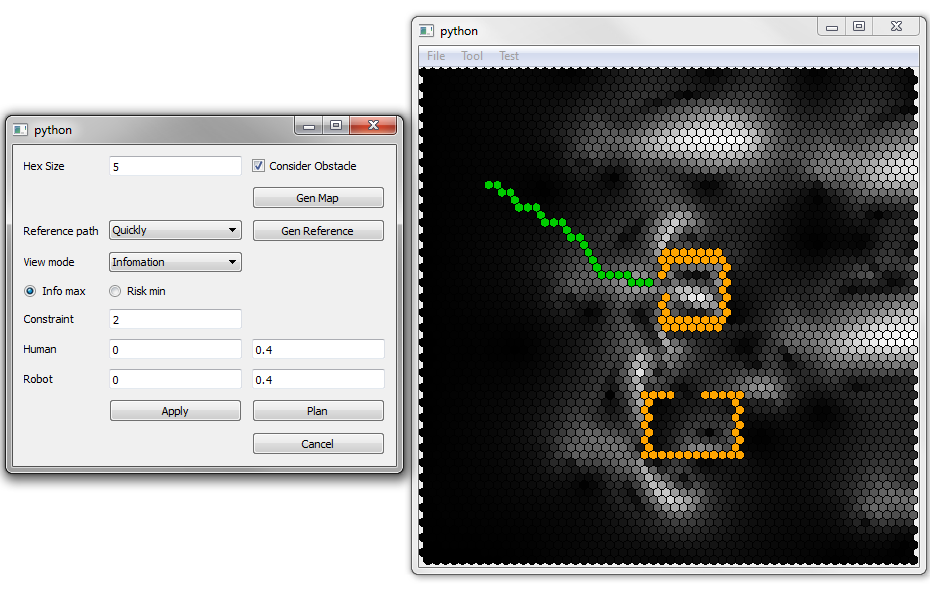
\includegraphics[width = \textwidth]{./screenshot/quickly_reference_path.png}
\end{figure}

\column{0.35\textwidth}
\begin{minipage}{\textwidth}
\begin{itemize}
\item \textbf{Start point}
\item \textbf{End point}
\end{itemize}
\end{minipage}
\end{columns}

\end{frame}

\begin{frame}{Reference path}{Safely}

\begin{columns}
\column{0.65\textwidth}
\begin{figure}
\centering
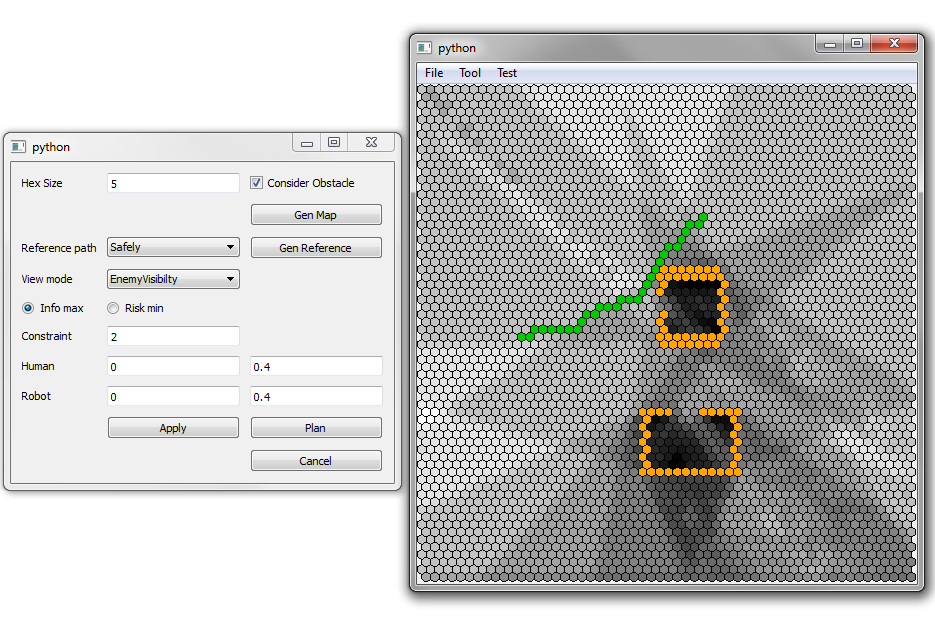
\includegraphics[width = \textwidth]{./screenshot/safely_reference_path.png}
\end{figure}

\column{0.35\textwidth}
\begin{minipage}{\textwidth}
\begin{itemize}
\item \textbf{Start point}
\item \textbf{End point}
\end{itemize}
\end{minipage}
\end{columns}

\end{frame}

\begin{frame}{Path planning}{Maximize information}

\begin{columns}
\column{0.7\textwidth}
\begin{figure}
\centering
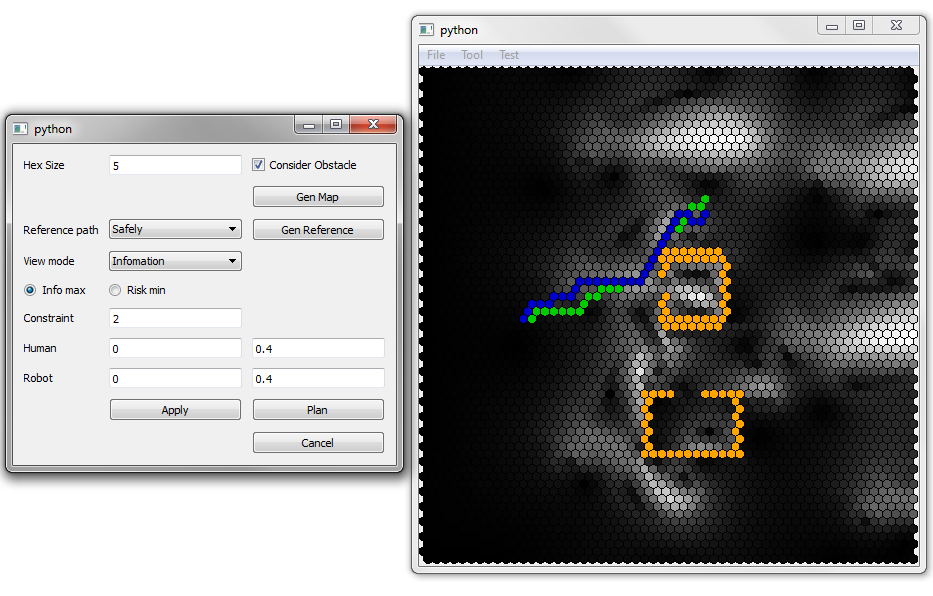
\includegraphics[width = \textwidth]{./screenshot/info_max_path.png}
\end{figure}

\column{0.3\textwidth}
\begin{minipage}{\textwidth}
\end{minipage}
\end{columns}

\end{frame}

\begin{frame}{Path planning}{Minimize risk}

\begin{columns}
\column{0.7\textwidth}
\begin{figure}
\centering
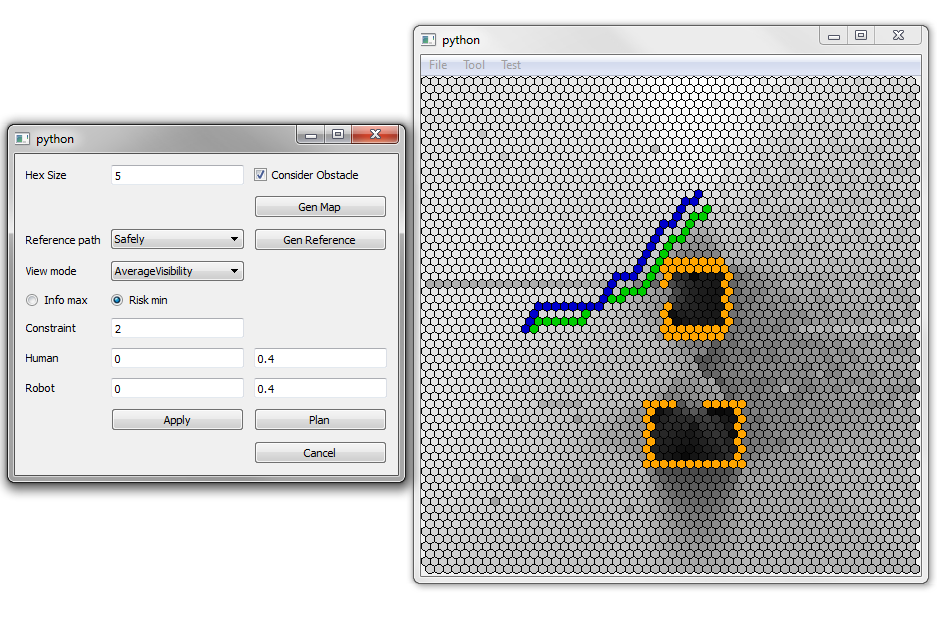
\includegraphics[width = \textwidth]{./screenshot/risk_min_path.png}
\end{figure}

\column{0.3\textwidth}
\begin{minipage}{\textwidth}
\end{minipage}
\end{columns}

\end{frame}

\section{Execution}

\begin{frame}{Path}{Waypoint sequence}

\begin{columns}
\column{0.6\textwidth}
\begin{figure}
\centering
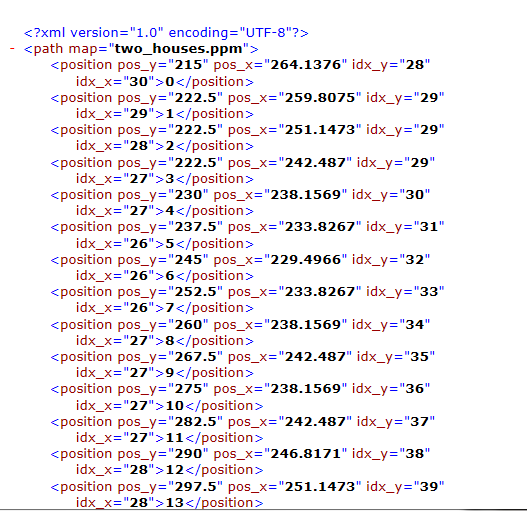
\includegraphics[width = \textwidth]{./screenshot/planned_path.png}
\end{figure}

\column{0.4\textwidth}
\begin{minipage}{\textwidth}
\end{minipage}
\end{columns}

\end{frame}

\begin{frame}{Path}{Simulator execution}

\begin{columns}
\column{0.6\textwidth}
\begin{figure}
\centering
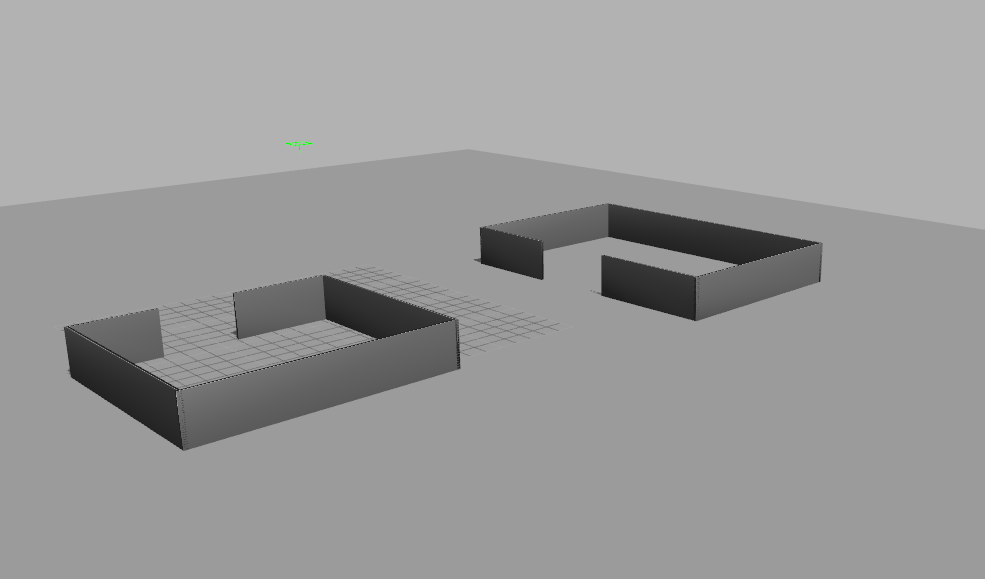
\includegraphics[width = \textwidth]{./screenshot/Gazebo_running.png}
\end{figure}

\column{0.4\textwidth}
\begin{minipage}{\textwidth}
\begin{figure}
\centering
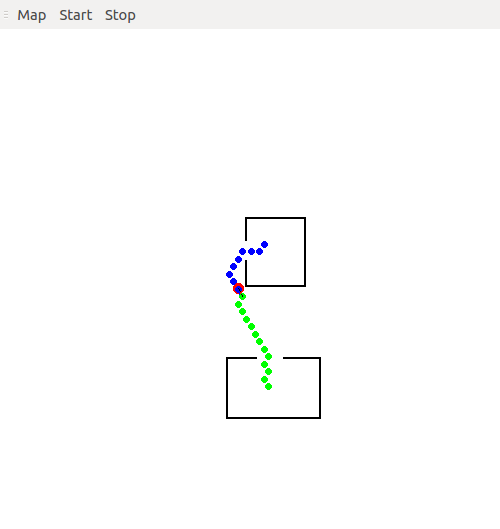
\includegraphics[width = \textwidth]{./screenshot/path_execution.png}
\end{figure}
\end{minipage}
\end{columns}

\end{frame}



% All of the following is optional and typically not needed. 

\end{document}


